\documentclass[25pt, a0paper, portrait]{tikzposter}
\usepackage[utf8]{inputenc}
 
\title{Fast-Slow Dynamics}
\author{Jonna, Kieran, Tom }
\date{14/12/2018}
\institute{MIGSAA}
 
\usepackage{blindtext}
\usepackage{comment}
\usepackage{amsmath}
%\usepackage{proj1}
\usetheme{Board}
 
\begin{document}
 
\maketitle
 
\block{~}
{

Fast- Slow systems are systems of differential equations that can be viewed on two different time scales, which are separated by a parameter.
These systems are generally of the form
\begin{equation*} 
\begin{cases}
x' &=\frac{dx}{dt}= f(x,y,\lambda, \epsilon),\\
y' &= \frac{dy}{dt}= \epsilon g( x,y, \lambda, \epsilon),
\end{cases}\label{FastS}
\end{equation*}
which is known as the fast system.
Using a scaling for the time, $t = \frac{\tau}{\epsilon} $, we find that this can be rewritten as
\begin{align*}
\begin{cases}
\epsilon \dot{x} &= \epsilon \frac{dx}{d \tau} = f(x,y,\lambda, \epsilon),\\
\dot{y} & = \frac{dy}{d \tau} =  g( x,y, \lambda, \epsilon),
\end{cases}\label{SlowS}
\end{align*}
which is called the slow system.
}
 
\begin{columns}
    \column{0.4}
    \block{Van der Pol System}
{Fast System:
\begin{equation*}\label{fastsystem}
    \begin{cases} x'=y-\frac{x^3}{3}+x\\
    y'=-\epsilon x,
    \end{cases}
\end{equation*}
Slow System: 
\begin{equation*}\label{slowsystem}
    \begin{cases} \epsilon \dot{x}=y-\frac{x^3}{3}+x\\
    \dot{y}=-x,
    \end{cases}
\end{equation*}
}
\block{Singular Limit}
{
Layer Problem:
\begin{equation*}\label{fastsystem0}
    \begin{cases} x'=y-\frac{x^3}{3}+x,\\
    y'=0,
    \end{cases}
\end{equation*}
Reduced Problem:
\begin{equation*}\label{slowsystem0}
    \begin{cases} 0=y-\frac{x^3}{3}+x:=f,\\
    \dot{y}=-x.
    \end{cases}
\end{equation*}

}
 
    \column{0.6}
    \block{Phase Portrait: Van der Pol System}
{
\begin{tikzfigure}[h!]
	\centering
	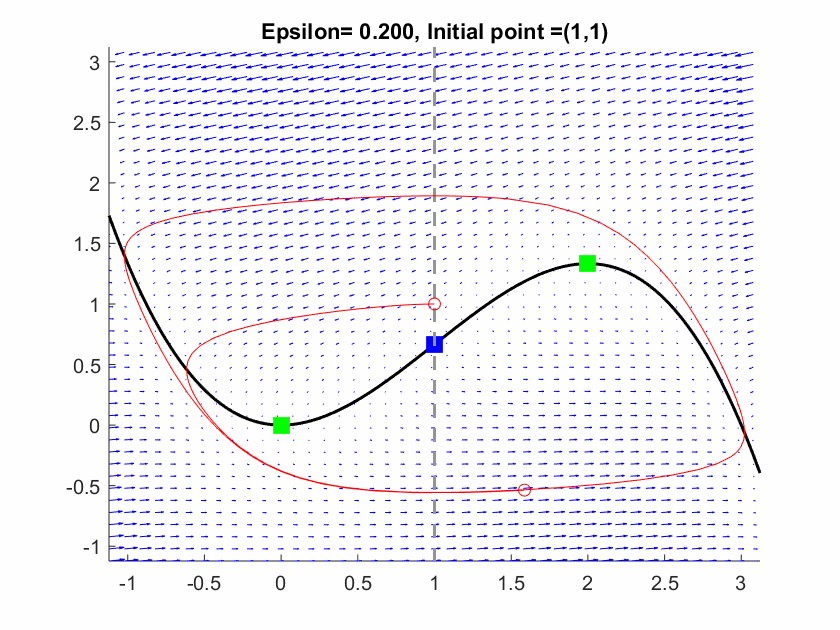
\includegraphics[height=20cm,width=26cm]{Posterpic1.jpg}
	%\caption{The reduced flow where a) $\lambda=0$ and b) $\lambda>0$.}
	%label{fig: Canard Point}
\end{tikzfigure}
}
    \block{Phase Portrait: Singular Limit}
{
\begin{tikzfigure}[h!]
	\centering
	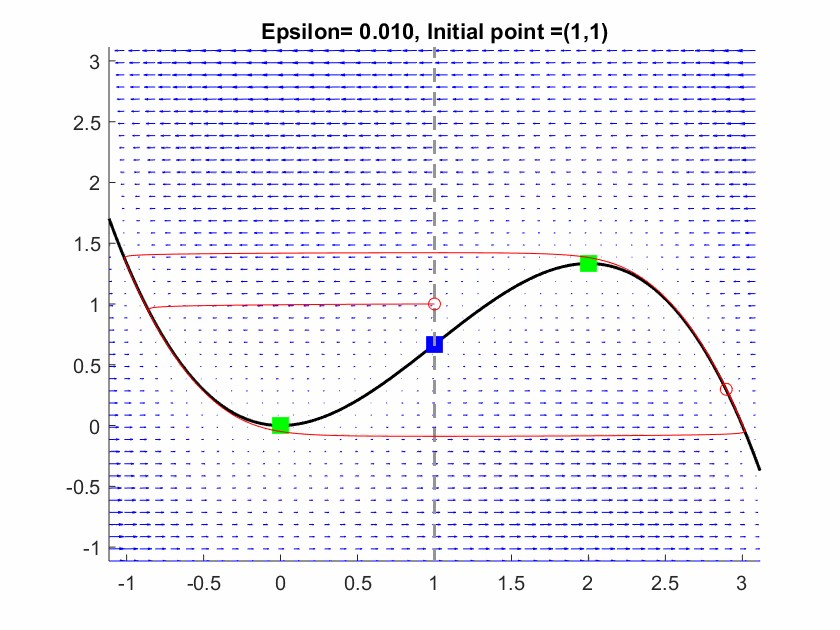
\includegraphics[height=20cm,width=26cm]{Posterpic2.jpg}
	%\caption{The reduced flow where a) $\lambda=0$ and b) $\lambda>0$.}
	%label{fig: Canard Point}
\end{tikzfigure}}

\end{columns}
 
\begin{columns}
    \column{0.5}
    \block{Canards}
    {Something
    }
    \column{0.5}
    \block{MMOs}{Pictures}
\end{columns}
 
\end{document}